% 2009 年山东卷理科第 19 题：得分 ξ 的分布列表头。
% 来源 PDF：普通高考/2009/2009山东理.pdf，SHA256 6c3546f276b37d6ff4fa1a8cdf77e8356b8a4c0e713e9e5485bb47fcd5ed660f
% 原页：第 2 页（A3 三栏）第 1 栏中部，印刷页 546。
% 重绘依据：两行五列表，上行 ξ 取 0、2、3、4、5，下行概率依次 0.03、p1、p2、p3、p4。
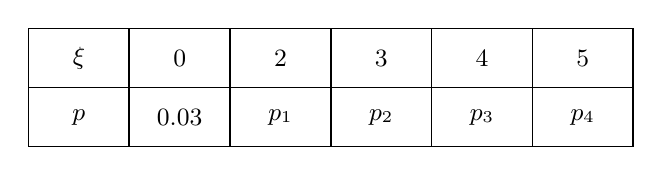
\begin{tikzpicture}[scale=1.0, semithick, every node/.style={inner sep=3.5pt, font=\small}]
  \draw (0,0) rectangle (7.68,-1.5);
  \draw (0,-0.75) -- (7.68,-0.75);
  \foreach \x in {1.28, 2.56, 3.84, 5.12, 6.4} {
    \draw (\x,0) -- (\x,-1.5);
  }
  \node at (0.64,-0.375) {$\xi$};
  \node at (1.92,-0.375) {$0$};
  \node at (3.2,-0.375) {$2$};
  \node at (4.48,-0.375) {$3$};
  \node at (5.76,-0.375) {$4$};
  \node at (7.04,-0.375) {$5$};
  \node at (0.64,-1.125) {$p$};
  \node at (1.92,-1.125) {$0.03$};
  \node at (3.2,-1.125) {$p_1$};
  \node at (4.48,-1.125) {$p_2$};
  \node at (5.76,-1.125) {$p_3$};
  \node at (7.04,-1.125) {$p_4$};
\end{tikzpicture}
